% afterhours7.tex - Afer Hours Week 7
\chapter{After Hours Week 7}
\section{``Instant Website''}
\subsection{Brewing a website - in an instant}
We have spoken a little about other tools which are supplied with Git.
One of those is the \indexgit{instaweb} tool.
This tool allows you to spawn a web service quickly and easily, using a web daemon of your choice.
If you have never played with web services before it would be worth spending a few minutes understanding a little about how web daemons work.
This tool is not available on the Windows platform, but it can be used on both MacOS and Linux.

\emph{Instaweb} allows us to browse our repository from the comfort of a web browser.
We also have another benefit to running this from a web server.
We can allow people to access our repository to look around without giving them the ability to change anything or make any commits.

Before we run \texttt{git instaweb}, we need to ensure that we have a web daemon available to us.
\emph{Instaweb} automatically creates a configuration file for the web daemon of your choice, runs the daemon on a custom network port,
and loads a browser automatically pointing to the URL of the web instance you have just configured.
On our example machine, we have installed \index{lighttpd}lighttpd as our choice of web daemon.
Once again it is advised to understand the implications of this before you do it.
On Ubuntu, this can be installed by running \texttt{apt-get install lighttpd}.

\begin{code}
john@satsuki:~/coderepo$ git instaweb
john@satsuki:~/coderepo$ 
\end{code}

The tool is invoked by running \texttt{git instaweb} and when started, you should be presented with a browser as pictured below.
In our case, lighttpd has been installed, and so Git will use that as its daemon.
Firefox is also the default browser on this machine and so this is the browser that Git will choose to display the web page in.

\begin{figure}[hbt]
\centering
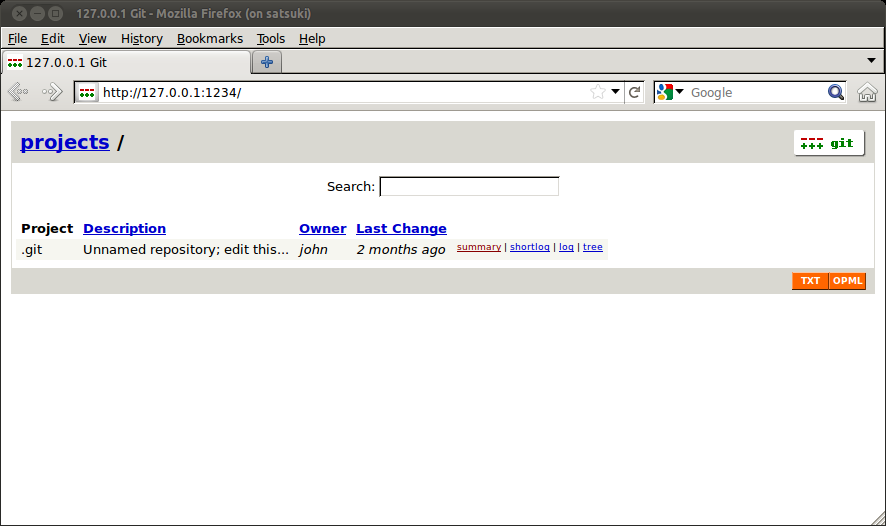
\includegraphics[width=10cm]{images/f-af7-d1.png}
\caption{Instaweb's default page}
\end{figure}

The first thing to notice is that the description of the repository is unhelpful.
In Figure 1, it is shown as \texttt{Unnamed repository; edit this...}.
It is easy to rectify this, by editing the \texttt{.git/description} file.
We are going to use the \texttt{echo} command from Linux, as we have throughout the book.

\begin{code}
john@satsuki:~/coderepo$ echo "Our test repository" > .git/description 
john@satsuki:~/coderepo$ 
\end{code}

On refreshing the page, the description will be updated.
The next thing to notice is the url.
The screenshot shows our url to be \texttt{http://127.0.0.1:1234/}, where \texttt{127.0.0.1} is the local address of our Git machine and \texttt{1234} is the port.

Before we start taking a look around the web interface, we should learn how to end the \emph{Instaweb} session.
If we close the web browser, it does not end the \emph{Instaweb} process.
In fact, we could load up firefox again, type in the URL \texttt{http://127.0.0.1:1234/} and return to the home page of our Git repository.
To close the instance of \emph{Instaweb} we run the following;

\begin{code}
john@satsuki:~/coderepo$ git instaweb --stop
john@satsuki:~/coderepo$ 
\end{code}

Now would be a good time to take a quick look at what running \texttt{git instaweb} has done to our repository.
